\documentclass[11pt,twocolumn]{article}

% --- Codificación y lenguaje ---
\usepackage[T1]{fontenc}
\usepackage[utf8]{inputenc}
\usepackage[spanish]{babel}

% --- Matemática y fuentes ---
\usepackage{amsfonts, amssymb, amsthm,amsmath}
\usepackage{derivative}
% \usepackage{physics} % No se usa en este informe; evitar conflicto con siunitx (\qty).

% --- Ajustes de composición en dos columnas ---
% Evitan avisos de Underfull \hbox/\vbox producidos por líneas estrechas,
% títulos largos, enlaces y expresiones matemáticas dentro del formato twocolumn.
\setlength{\emergencystretch}{3em}
\hbadness=10000
\vbadness=10000
\hfuzz=20pt
\vfuzz=20pt
\raggedbottom

% --- Gráficos y tablas ---
\usepackage{graphicx}
\usepackage{caption}        % <-- primero caption
\usepackage{subcaption}     % <-- luego subcaption
\usepackage{booktabs}
\usepackage{ulem} 
\usepackage{siunitx}

% --- Varios útiles ---
\usepackage[margin=2cm]{geometry}
\usepackage{enumitem}
\usepackage{csquotes}
\usepackage{cuted}          % para elementos a dos columnas (opcional)
\usepackage{stackrel}
%\usepackage{microtype}      % cargar una sola vez
\usepackage{float}
\usepackage{placeins}
\usepackage{multirow}
% \usepackage{nameref}      % NO necesario: hyperref ya define \nameref
\usepackage[dvipsnames]{xcolor}
\usepackage{tikz}
\usetikzlibrary{calc}

% --- Bibliografía (BibTeX + apacite) ---
\usepackage[backend=biber,style=apa,language=spanish]{biblatex}
\addbibresource{references.bib} % tu archivo original con @online
% Mejor corte de URLs y entradas largas en la bibliografía.
\setcounter{biburllcpenalty}{7000}
\setcounter{biburlucpenalty}{8000}
\setcounter{biburlnumpenalty}{9000}
\AtBeginBibliography{\raggedright\sloppy}


% --- Hipervínculos (casi al final) ---
\usepackage[
  colorlinks=true,
  linkcolor=black, urlcolor=black, citecolor=black, filecolor=black,
  pdfborder={0 0 0}
]{hyperref}
% --- Colores para hipervínculos (citas en azul) ---
\hypersetup{
  colorlinks=true,
  linkcolor=black,      % refs, índice
  urlcolor=Blue,
  citecolor=Blue   % color del link de la cita
}

% --- Forzar que TODA la cita (no solo el link) salga en color
\makeatletter
\let\orig@cite\cite
\renewcommand{\cite}[1]{\textcolor{Blue}{\orig@cite{#1}}}

% Si en el texto usaste \citeA (cita textual tipo Autor (Año)),
% la convertimos también a formato entre paréntesis y color:
% --- Citas parentéticas y en color, compatible con apacite o biblatex ---
\makeatletter
% ¿Existe \citeA (apacite)? Si no, asumimos biblatex.
\@ifundefined{citeA}{%
  % --------- rama biblatex ---------
  % Si existe \parencite, la coloreamos y mapeamos \cite / \citeA a paréntesis:
  \@ifundefined{parencite}{}{%
    \let\orig@parencite\parencite
    \renewcommand{\parencite}[1]{\textcolor{Blue}{\orig@parencite{#1}}}
    \renewcommand{\cite}[1]{\parencite{#1}}      % \cite -> (Autor, Año)
    \providecommand{\citeA}[1]{\parencite{#1}}   % por si quedó \citeA en el texto
    % (Opcional) forzar \textcite también a parentético:
    % \let\orig@textcite\textcite
    % \renewcommand{\textcite}[1]{\parencite{#1}}
  }%
}{%
  % --------- rama apacite ---------
  \let\orig@cite\cite
  \renewcommand{\cite}[1]{\textcolor{Blue}{\orig@cite{#1}}} % color a (Autor, Año)
  % Hacer que \citeA (Autor (Año)) también salga parentético y en color:
  \let\orig@citeA\citeA
  \renewcommand{\citeA}[1]{\textcolor{Blue}{\orig@cite{#1}}}
}
\makeatother

\begin{document}

\begin{tikzpicture}[remember picture,overlay]
  \node[anchor=north east, inner sep=0pt]
    at ($(current page.north east)+(-1.8cm,-1.2cm)$)
    {
\includegraphics[height=2.8cm]{UdeC_logo_azul.png}};
\end{tikzpicture}

\begin{strip}
\begin{center}
\vspace*{-5\baselineskip}
{\Large \textbf{Universidad de Concepción}}\\[-2pt]
\small Facultad de Ciencias Físicas y Matemáticas\\[-2pt]
\small \textit{Laboratorio II (510352-1)}\\[4pt]

{\Large \bfseries Informe 4: Intercambio de energía mecánica}\\
[2pt]
{\Large \bfseries en un sistema cuerpo–resorte oscilando}\\
[2pt]
\small Profesor: Paulraj Manidurai\\[-2pt]
\small F. Contreras M., J. Rosas S., J. Chandia V., M. Díaz S., M. Fierro S.\\[-2pt]
\small Concepción, Chile — 20 de octubre de 2025
\end{center}
\vspace{0.5\baselineskip}
\hrule
\vspace{0.8\baselineskip}

% ===========================
% 0. Abstract.
% ===========================

\begin{abstract}
Se estudiaron \textbf{dos} sistemas masa–resorte en dos etapas complementarias. En la \textbf{Primera experiencia} (estática) se determinó la constante elástica $k$ de cada resorte a partir de la relación lineal fuerza–elongación. En la \textbf{Segunda experiencia} (dinámica) se analizan las oscilaciones alrededor del equilibrio, \textbf{usando la amplitud definida a partir de las posiciones extremas}, mostrando el intercambio entre energía potencial gravitatoria y elástica, con pérdidas no conservativas menores. Se documentan procedimientos y marco teórico mínimos para la reproducibilidad del análisis.
\end{abstract}

\noindent\rule{\textwidth}{0.4pt}\par\vspace{0.3cm}
\end{strip}

% ===========================
% 1. Objetivos.
% ===========================

\section{Objetivo.}

\begin{itemize}
    \item Determinar la constante elástica $k$ de \textbf{cada} resorte en régimen lineal mediante mediciones estáticas $F$–$\Delta x$. 
    \item Evaluar, para ambos resortes, el intercambio $E_p^{\text{grav}}\leftrightarrow E_p^{\text{elast}}$ durante oscilaciones libres alrededor del equilibrio, \textbf{usando $\Delta y$ definida desde $y_{\text{sup}}$ e $y_{\text{inf}}$} y las $k$ estáticas correspondientes.

\end{itemize}

% ===========================
% 2. Introducción.
% ===========================
\section{Introducción.}

Los sistemas masa–resorte constituyen un modelo estándar para el estudio de respuestas elásticas, equilibrio estático y transferencia de energía mecánica \cite{HallidayResnick}.En la \textbf{primera experiencia} del presente trabajo se contrasta la \emph{ley de Hooke} en régimen lineal ($F = k\,x$) mediante mediciones estáticas de elongación, con el fin de estimar la constante elástica $k$ del resorte \cite{SerwayHooke}. En la \textbf{segunda experiencia}, se analizan las oscilaciones libres de la masa colgante y se registran las elongaciones extremas respecto del equilibrio, comparando la energía potencial gravitatoria $E_p^{\text{grav}} = mgh$ con la energía potencial elástica $E_p^{\text{elast}} = \tfrac{1}{2}kx^2$ \cite{TiplerEnergia, FeynmanLectures}. En el resto del informe se adopta un eje vertical $y$ positivo hacia abajo, con $y=0$ en el equilibrio; por tanto, la energía potencial gravitatoria relativa al equilibrio se escribe como $E_p^{\text{grav}}(y)=-mg\,y$ (equivalente a $mgh$ tomando $h=-y$). El montaje experimental básico se muestra en la Figura~\ref{fig:montaje_resorte}, donde se representa la posición inicial del resorte y su deformación ante la carga aplicada.

% ===========================
% 3. Marco teórico.
% ===========================
\section{Marco teórico.}

\subsection{Ley de Hooke y régimen lineal}

Para elongaciones moderadas, la fuerza recuperadora del resorte se aproxima por
\begin{equation*}
    F = k\,x,
\end{equation*}
donde $F$ es la fuerza aplicada, $x$ la elongación respecto a la longitud natural del resorte, y $k$ la constante elástica \cite{SerwayHooke}. Este modelo es válido únicamente en el régimen elástico lineal; fuera de dicho rango pueden aparecer no linealidades, deformaciones plásticas o cargas residuales \cite{HallidayResnick}.

\subsection{Equilibrio estático de la masa colgante}

Cuando una masa $m$ se cuelga del resorte y se deja en reposo, se alcanza un estado de equilibrio en el cual la fuerza elástica compensa exactamente el peso:
\begin{equation*}
    k\,x_{\mathrm{eq}} = m\,g 
\quad \Rightarrow \quad 
k = \frac{m\,g}{x_{\mathrm{eq}}}.
\end{equation*}
Este principio permite estimar $k$ experimentalmente a partir de pares $(m, x_{\mathrm{eq}})$, y se refina mediante ajuste lineal entre $F = mg$ y $x$ \cite{HallidayResnick}.

\subsection{Energías potenciales y referencia de alturas}

Tomando como referencia el punto de equilibrio ($y=0$) y un eje vertical $y$ positivo hacia abajo (coherente con la escala de lectura), las energías potenciales involucradas en el sistema masa–resorte se expresan como
\begin{equation*}
    E_p^{\text{grav}}(y) = -m g\, y,
    \qquad
    E_p^{\text{elast}}(x) = \tfrac{1}{2}k x^2,
\end{equation*}
donde $x$ es la elongación respecto de la longitud natural del resorte. 
En ausencia de pérdidas, la energía mecánica total
\begin{equation*}
    E = E_p^{\text{grav}} + E_p^{\text{elast}} + E_c
\end{equation*}
permanece constante a lo largo del movimiento \cite{TiplerEnergia}. Desde una perspectiva conceptual, este intercambio energético entre la gravedad y la elasticidad es un ejemplo clásico de sistemas conservativos \cite{FeynmanLectures}.

\subsection{Extremos de la oscilación y consistencia energética}

En los extremos de la oscilación (elongación máxima superior e inferior), la velocidad instantánea es nula ($E_c = 0$), por lo que
\begin{equation*}
    E_{\max} = -m g \,y_{\max} + \tfrac{1}{2}k x_{\max}^2,
\end{equation*}
coherente con la convención $y$ positiva hacia abajo y $E_p^{\text{grav}}(y)=-mg\,y$.

Comparar $E_{\max}$ superior e inferior permite evaluar la conservación de energía. Discrepancias pueden atribuirse a amortiguamiento, fricción interna o histéresis\footnote{La histéresis representa la tendencia de un material a conservar una de sus propiedades, en ausencia del estímulo que la ha generado.} del resorte \cite{MITOscilaciones}.

\subsection{Intercambio de energías en torno al equilibrio}

Adoptamos un eje vertical $y$ positivo hacia abajo y $y=0$ en equilibrio. Denotamos por $\Delta>0$ la semidiferencia entre extremos, de modo que
\begin{equation*}
    y_{\text{sup}}=-\Delta,\qquad y_{\text{inf}}=+\Delta.
\end{equation*}
Sea $y_L=\frac{mg}{k}$ la elongación estática del resorte respecto de su longitud natural; la elongación en una posición genérica $y$ es $x=y+y_L$.

\paragraph{Energía potencial gravitatoria.}
En el extremo superior ($y_{\text{sup}}=-\Delta$):
\begin{align*}
    E_p^{\text{grav, sup}}&=-mg\,y_{\text{sup}} \\[4pt]
    &=-mg(-\Delta)\\[4pt]
    &=+mg\,\Delta.
\end{align*}
En el extremo inferior ($y_{\text{inf}}=+\Delta$):
\begin{align*}
    E_p^{\text{grav, inf}}&=-mg\,y_{\text{inf}} \\[4pt]
    &=-mg(+\Delta) \\[4pt]
    &=-mg\,\Delta.
\end{align*}
Por tanto,
\begin{align*}
    \Delta E_p^{\text{grav}}
&=E_p^{\text{grav, inf}}-E_p^{\text{grav, sup}}\\[4pt]
&=(-mg\,\Delta)-(+mg\,\Delta)\\[4pt]
&=-2mg\,\Delta.
\end{align*}

\paragraph{Energía potencial elástica.}
Como $x=y+y_L$, en los extremos
\begin{align*}
    x_{\text{sup}}&=y_{\text{sup}}+y_L=y_L-\Delta,\\[6pt]
    x_{\text{inf}}&=y_{\text{inf}}+y_L=y_L+\Delta,
\end{align*}
y
\begin{align*}
    E_p^{\text{elast, sup}}&=\tfrac12 k (y_L-\Delta)^2, \\[6pt]
    E_p^{\text{elast, inf}}&=\tfrac12 k (y_L+\Delta)^2.
\end{align*}
Luego,
\begin{align*}
    \Delta E_p^{\text{elast}}
    &=E_p^{\text{elast, inf}}-E_p^{\text{elast, sup}} \\[6pt]
    &=\tfrac12 k\big[(y_L+\Delta)^2-(y_L-\Delta)^2\big] \\[6pt]
    &=2k\,y_L\,\Delta.
\end{align*}

Usando la condición de equilibrio $k\,y_L=mg$,
\begin{equation*}
    \Delta E_p^{\text{elast}}=2mg\,\Delta
= -\,\Delta E_p^{\text{grav}}.
\end{equation*}
En suma, las variaciones de energía potencial gravitatoria y elástica son iguales en magnitud y opuestas en signo, por lo que la energía mecánica total se conserva en una oscilación ideal (sin pérdidas).

\begin{figure}
    \centering
    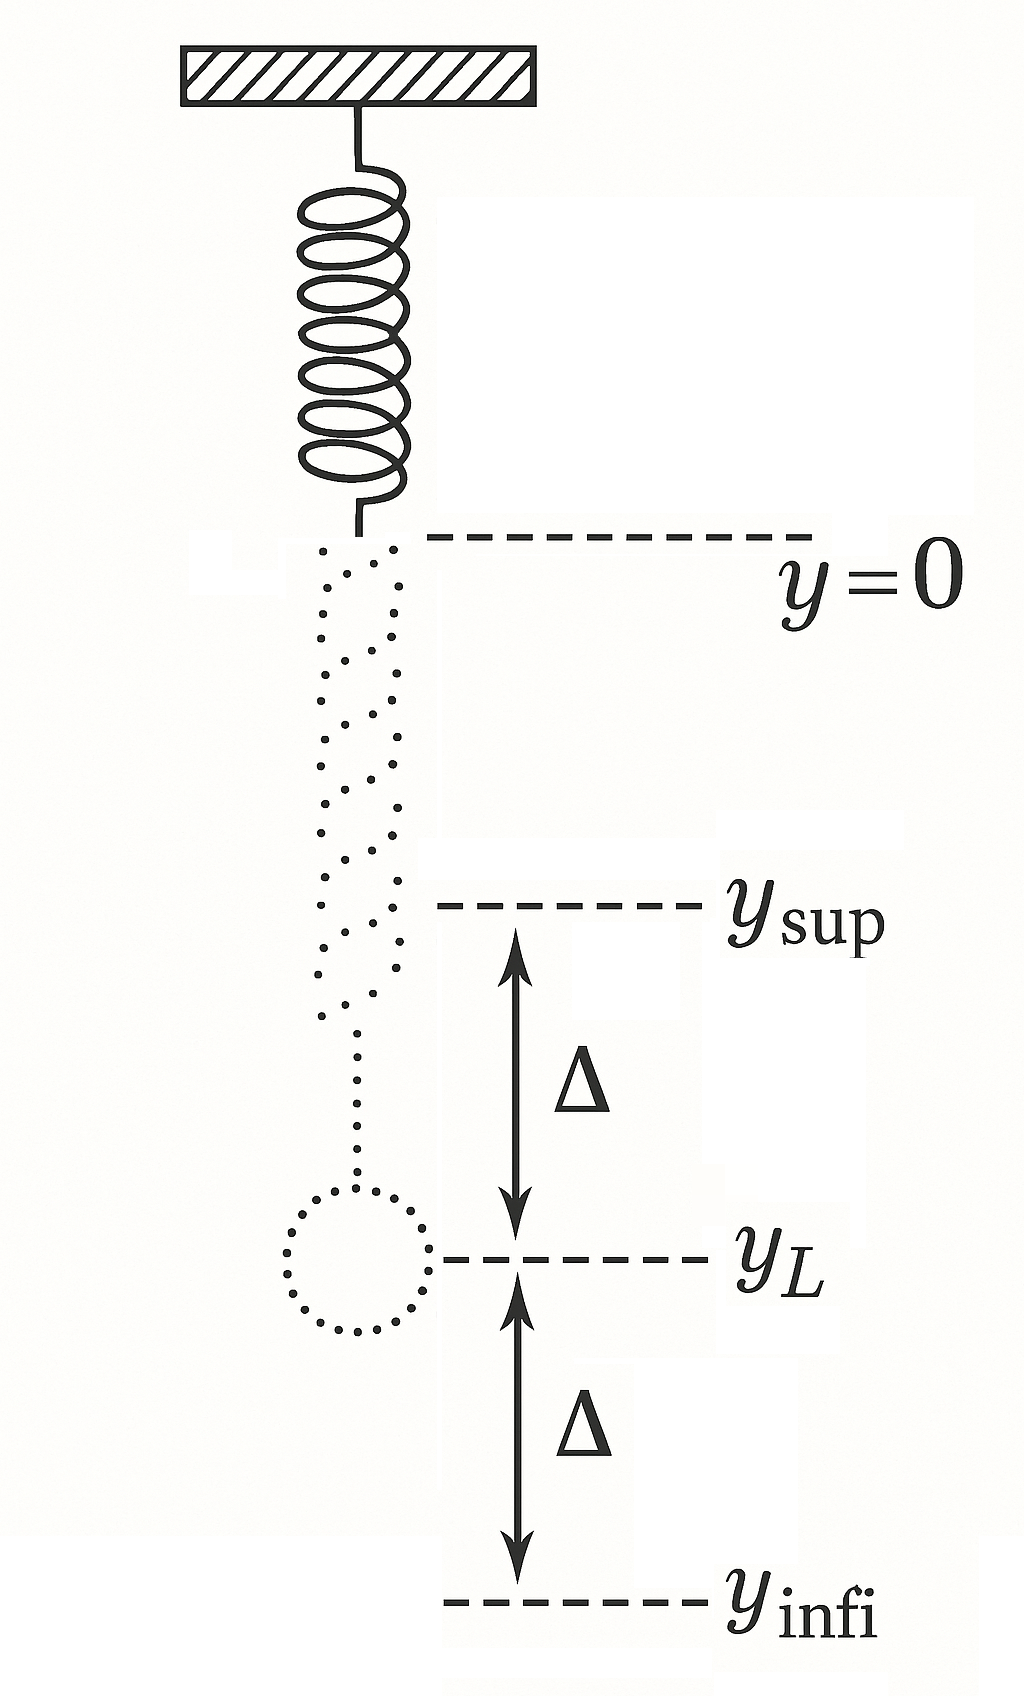
\includegraphics[width=0.5\linewidth]{figures/figure_1.png}
    \caption{Esquema del sistema masa–resorte. Se indican la posición de equilibrio $y = 0$, la longitud del resorte en equilibrio $y_L$, y las posiciones extremas superior e inferior separadas por la amplitud $\Delta$.}
    \label{fig:posiciones_resorte}
\end{figure}


% ===========================
% 4. Materiales:
% ===========================
\section{Materiales.}

El experimento se realizó utilizando un conjunto de elementos básicos para el estudio de sistemas elásticos en régimen estático y dinámico. Entre los principales componentes se incluyeron dos resortes helicoidales y masas patrón combinables de distintos valores, junto con instrumentos de sujeción y medición. Los materiales empleados se detallan a continuación:

\begin{itemize}
    \item \textbf{Dos resortes helicoidales} (constante elástica dentro del rango de laboratorio).
    \item \textbf{Juego de masas patrón combinables}: valores de $0.25~\mathrm{kg}$, $0.50~\mathrm{kg}$ y $1.00~\mathrm{kg}$.
    \item \textbf{Soporte universal con gancho superior}.
    \item \textbf{Regla milimetrada} de $1~\mathrm{m}$.
\end{itemize}

En la Figura~\ref{fig:materiales_resorte} se muestra parte del material utilizado, incluyendo las masas patrón y el instrumento de medición empleado para registrar las elongaciones del resorte.

\begin{figure}
    \centering
    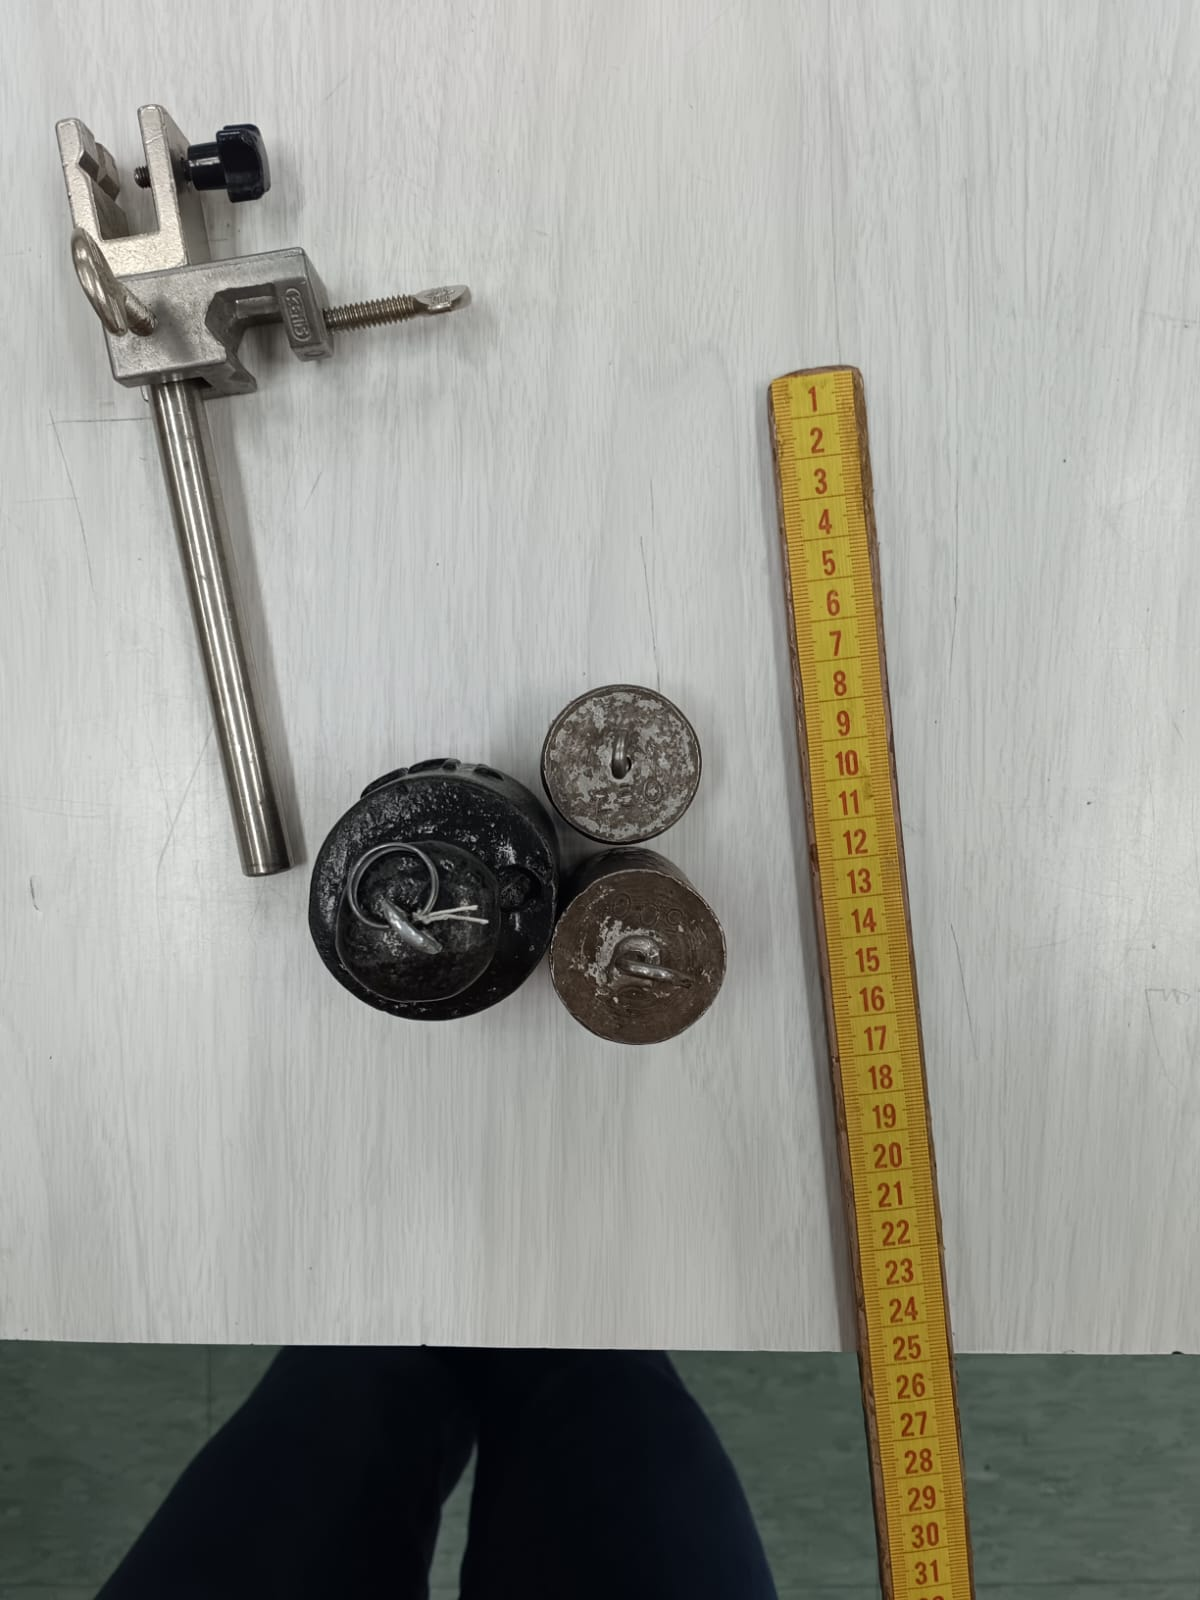
\includegraphics[width=0.8\linewidth]{materials/masas_regla.jpg}
    \caption{Juego de masas patrón y regla milimetrada utilizados para la medición de elongaciones en el sistema masa–resorte.}
    \label{fig:materiales_resorte}
\end{figure}

% ===========================
% 5. Primera experiencia.
% ===========================
\section{Primera experiencia.}
\label{sec:primera_experiencia}

En esta etapa se estudió la respuesta elástica de \textbf{los resortes} en régimen estático. En lugar de trabajar con la longitud natural del resorte, se adoptó como referencia la \textbf{posición del extremo libre sin carga} $x_i$ y, para cada masa $m$, se registró la lectura en equilibrio $x_f$ sobre la misma escala. La \textbf{elongación} se definió como $\Delta x = |x_f - x_i|$ y la \textbf{fuerza aplicada} como $F=mg$ (con $g=9.81~\mathrm{m/s^2}$). La Figura~\ref{fig:montaje_resorte} ilustra el esquema de medición y la definición de las magnitudes utilizadas.

\subsection{Procedimiento.}

\begin{enumerate}[leftmargin=*,itemsep=2pt,topsep=2pt]
    \item Con el \textbf{primer resorte} suspendido del soporte, y empleando una \textbf{regla milimetrada} fijada verticalmente como escala de referencia, se fijó la \emph{longitud de referencia} del extremo libre $x_i$ (elongación cero) en ausencia de masa.
    \item A continuación, se colgó una masa $m$ conocida y se esperó hasta que el sistema alcanzara el \emph{equilibrio estático}. Se registró la lectura del extremo libre $x_f$ sobre la misma regla y se calculó la elongación $\Delta x = |x_f - x_i|$.
    \item El procedimiento se repitió para un conjunto de masas crecientes (\textbf{al menos 4–8 valores}), evitando grandes deformaciones que excedieran el régimen lineal del resorte. Se reiteran los pasos anteriores con el \textbf{segundo resorte}.
    \item Para cada valor registrado, se asignó $F = mg$ como fuerza aplicada y se construyó la tabla de pares $(F, \Delta x)$ organizada en orden ascendente de fuerza.
    \item Posteriormente, se aplicó un ajuste por mínimos cuadrados al modelo $F = k\,\Delta x + b$. La pendiente del ajuste permitió estimar la constante elástica $k$, mientras que el intercepto $b$ cuantificó posibles \emph{offsets}\footnote{Deberia de esperarse $b\approx 0$, lo suficientemente despreciable}.
    \item Finalmente, se reportó el valor de $k \pm \Delta k$ y se conservaron las tablas y figuras necesarias para el análisis de resultados.
\end{enumerate}

El esquema de la Figura~\ref{fig:montaje_resorte} resume el procedimiento de medición: en (a) se observa la posición del extremo libre sin carga ($x_i$) alineada con la escala de la regla milimetrada, y en (b) la nueva lectura con masa y gancho ($x_f$), a partir de la cual se define la elongación $\Delta x = |x_f - x_i|$.

\begin{figure}
    \centering
    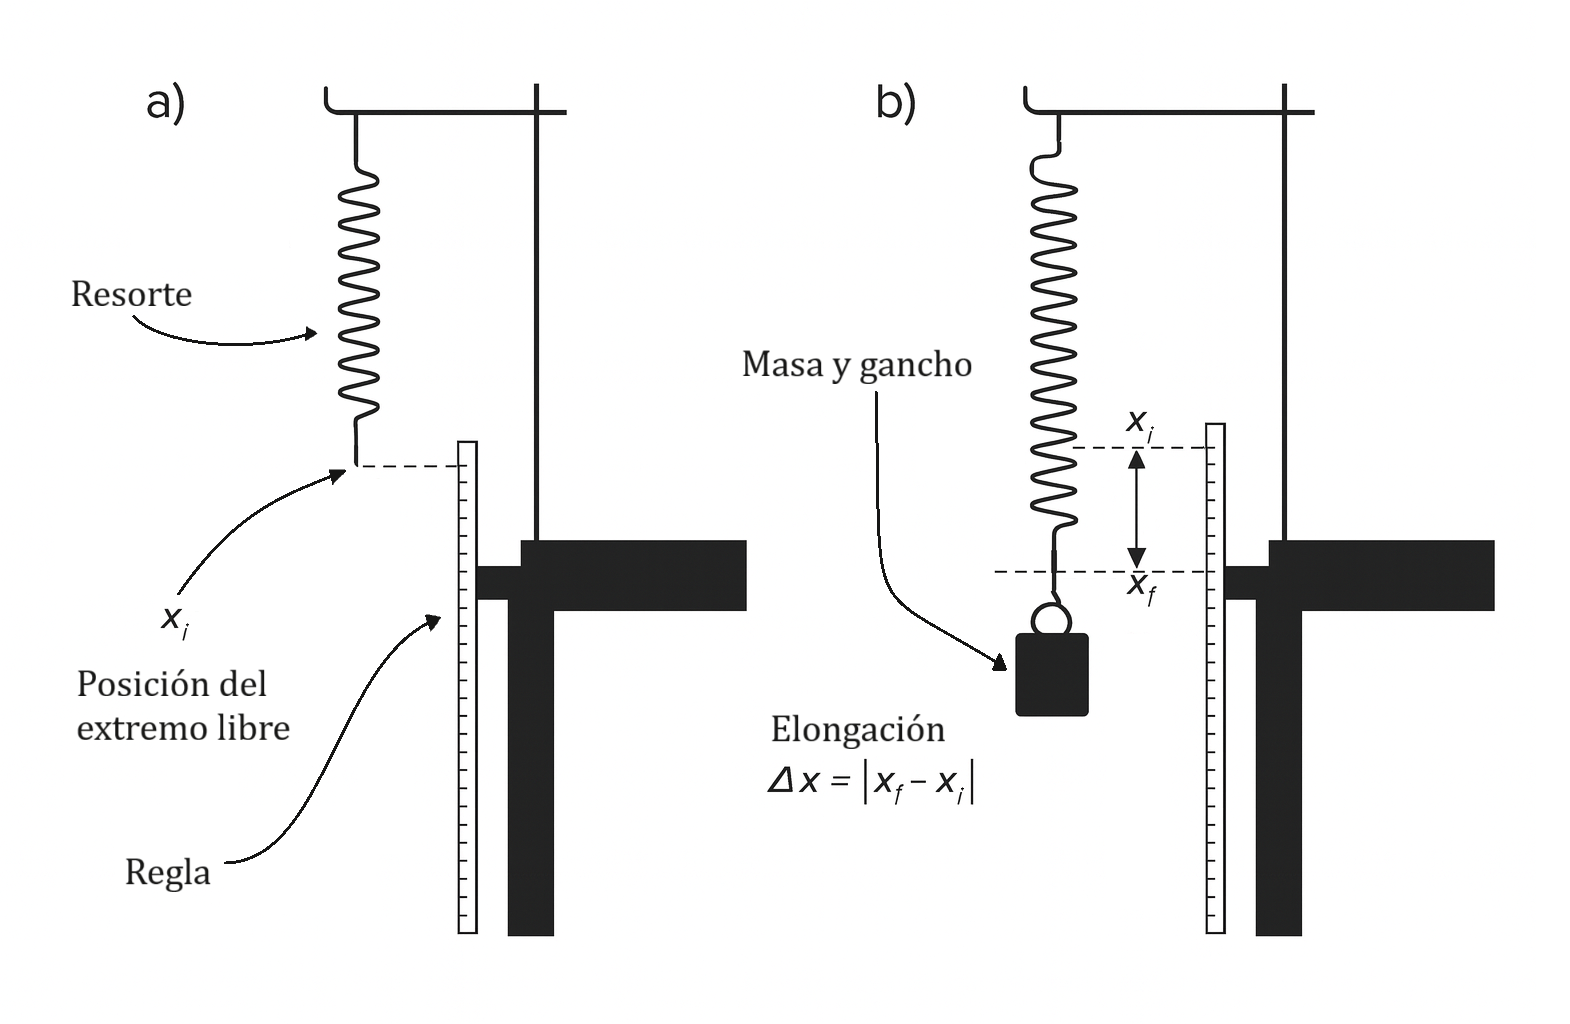
\includegraphics[width=1\linewidth]{figures/figure_2.png}
    \caption{Montaje para la determinación estática de $k$. (a) Resorte sin carga: $x_i$ es la lectura del extremo libre en la \textbf{regla milimetrada} fijada al soporte. (b) Resorte con masa y gancho: $x_f$ es la nueva lectura. La elongación se define como $\Delta x = |x_f - x_i|$.}
    \label{fig:montaje_resorte}
\end{figure}

\subsection{Reporte de datos.}

Todas las mediciones se realizaron con el sistema en \textbf{equilibrio estático}, leyendo directamente el extremo libre del resorte sobre una \textbf{regla milimetrada} fijada al soporte. Se reportan los pares \((\Delta x, F)\) en unidades SI, donde
\begin{align*}
    \Delta x &= |x_f - x_i|, \\[4pt]
    F &= m g \quad (g = 9.81~\mathrm{m/s^2}).
\end{align*}
Las masas corresponden a cuerpos individuales y a combinaciones simples, tal como se indica en la primera columna. 
Los datos se presentan en los \textbf{Cuadros}~\ref{tab:resorte1_parte1} y \ref{tab:resorte2_parte1}.

\begin{table}
\centering
\caption{Datos de fuerza $F$ y elongación $\Delta x$ para el \textbf{resorte 1} (Parte I).}
\label{tab:resorte1_parte1}
\begin{tabular}{|c|c|c|}
\hline
\textbf{Masa} (kg) & $\Delta x$ (m) & $F$ (N) \\ \hline
$2.50\times10^{-1}$ & $9.70\times10^{-2}$ & $2.45$ \\ \hline
$5.00\times10^{-1}$ & $1.76\times10^{-1}$ & $4.90$ \\ \hline
$7.50\times10^{-1}$ & $2.52\times10^{-1}$ & $7.35$ \\ \hline
$1.00$              & $3.32\times10^{-1}$ & $9.82$ \\ \hline
$1.25$              & $4.27\times10^{-1}$ & $12.2$ \\ \hline
$1.50$              & $5.03\times10^{-1}$ & $14.7$ \\ \hline
\end{tabular}
\end{table}

\begin{table}
\centering
\caption{Datos de fuerza $F$ y elongación $\Delta x$ para el \textbf{resorte 2} (Parte I).}
\label{tab:resorte2_parte1}
\begin{tabular}{|c|c|c|}
\hline
\textbf{Masa} (kg) & $\Delta x$ (m) & $F$ (N) \\ \hline
$1.50\times10^{-1}$ & $1.50\times10^{-1}$ & $1.64$ \\ \hline
$2.00\times10^{-1}$ & $2.00\times10^{-1}$ & $2.13$ \\ \hline
$2.50\times10^{-1}$ & $2.50\times10^{-1}$ & $2.62$ \\ \hline
$3.00\times10^{-1}$ & $3.00\times10^{-1}$ & $3.11$ \\ \hline
\end{tabular}
\end{table}


% ======================================================
% 6. Análisis de datos de la primera experiencia.
% ======================================================

\section{Análisis de datos de la primera experiencia.}
\label{sec:_analisis_primera_experiencia}

Dado el conjunto de datos $\{(\Delta x_i, F_i)\}_{i=1}^n$ obtenido en la Sección~\ref{sec:primera_experiencia}, se ajustó el modelo lineal
\begin{equation*}
    F(\Delta x) = k\,\Delta x + b
\end{equation*}
mediante \textbf{mínimos cuadrados ordinarios} (MCO). Para su cálculo y las variables utilizadas, revisar la Sección~\ref{sec:Apendice}. El código completo que genera las Figuras~\ref{fig:F_vs_dx_resorte1} y \ref{fig:F_vs_dx_resorte2}, además de calcular el ajuste lineal por MCO, puede consultarse en \textcolor{RoyalBlue}{\href{https://udeconce-my.sharepoint.com/:u:/g/personal/jrosas2022_udec_cl/EWfICfQ27DZBoIxNwYx8hZMBxiDXPreNW3fPDT-XkyFqbQ?e=jCc2ct}{este script}}.

\subsection{Representación gráfica de \texorpdfstring{$F$}{F} en función de la elongación \texorpdfstring{$\Delta x$}{Delta x}}
En las Figuras~\ref{fig:F_vs_dx_resorte1} y \ref{fig:F_vs_dx_resorte2} se muestran los datos $(\Delta x, F)$ en unidades SI y la recta de mejor ajuste para el primer y segundo resorte, respectivamente.
La ligera desviación del primer punto respecto de la recta para los datos $(\Delta x, F)$ del primer resorte (véase Figura~\ref{fig:F_vs_dx_resorte1}) es compatible con un pequeño desplazamiento de cero (\emph{offset}/precarga). La proporcionalidad $F\propto\Delta x$ se mantiene en el rango de trabajo identificado más abajo. 

\begin{figure}
    \centering
    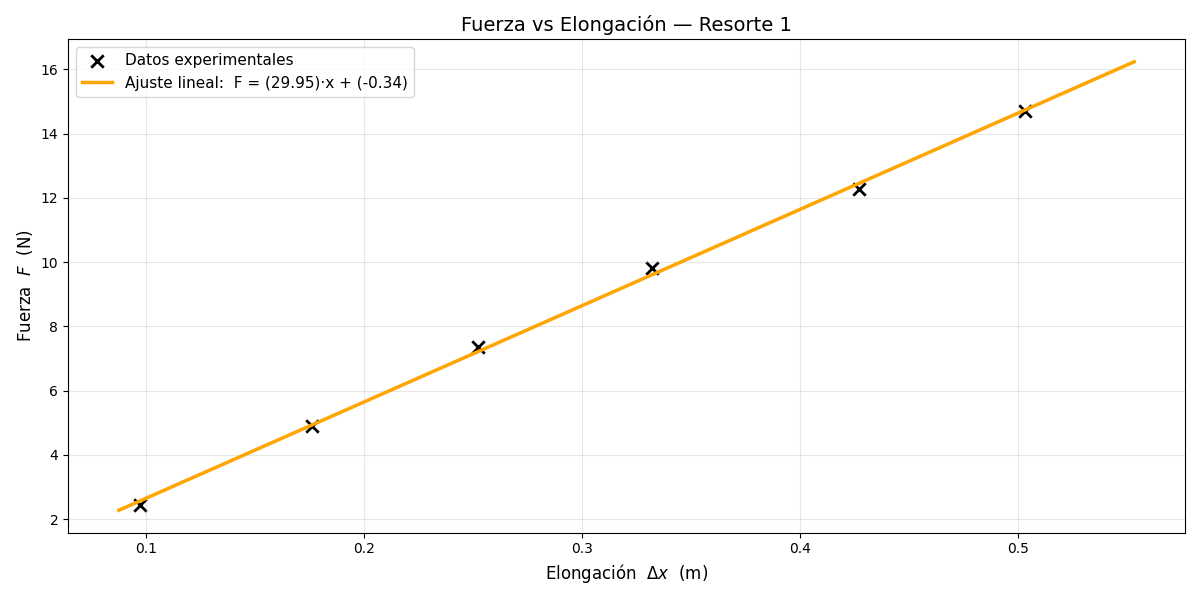
\includegraphics[width=\linewidth]{graphics/F_vs_DeltaX_resorte1.png}
    \caption{Fuerza $F$ en función de la elongación $\Delta x$ para el resorte 1. 
    Ajuste lineal $F = k\,\Delta x + b$ con 
    $k=(29{,}953)\,\left[\mathrm{N/m}\right]$, $b=(-0{,}339)\,\left[\mathrm{N}\right]$ y $R^2=0{,}9989$.}
    \label{fig:F_vs_dx_resorte1}
\end{figure}

\begin{figure}
    \centering
    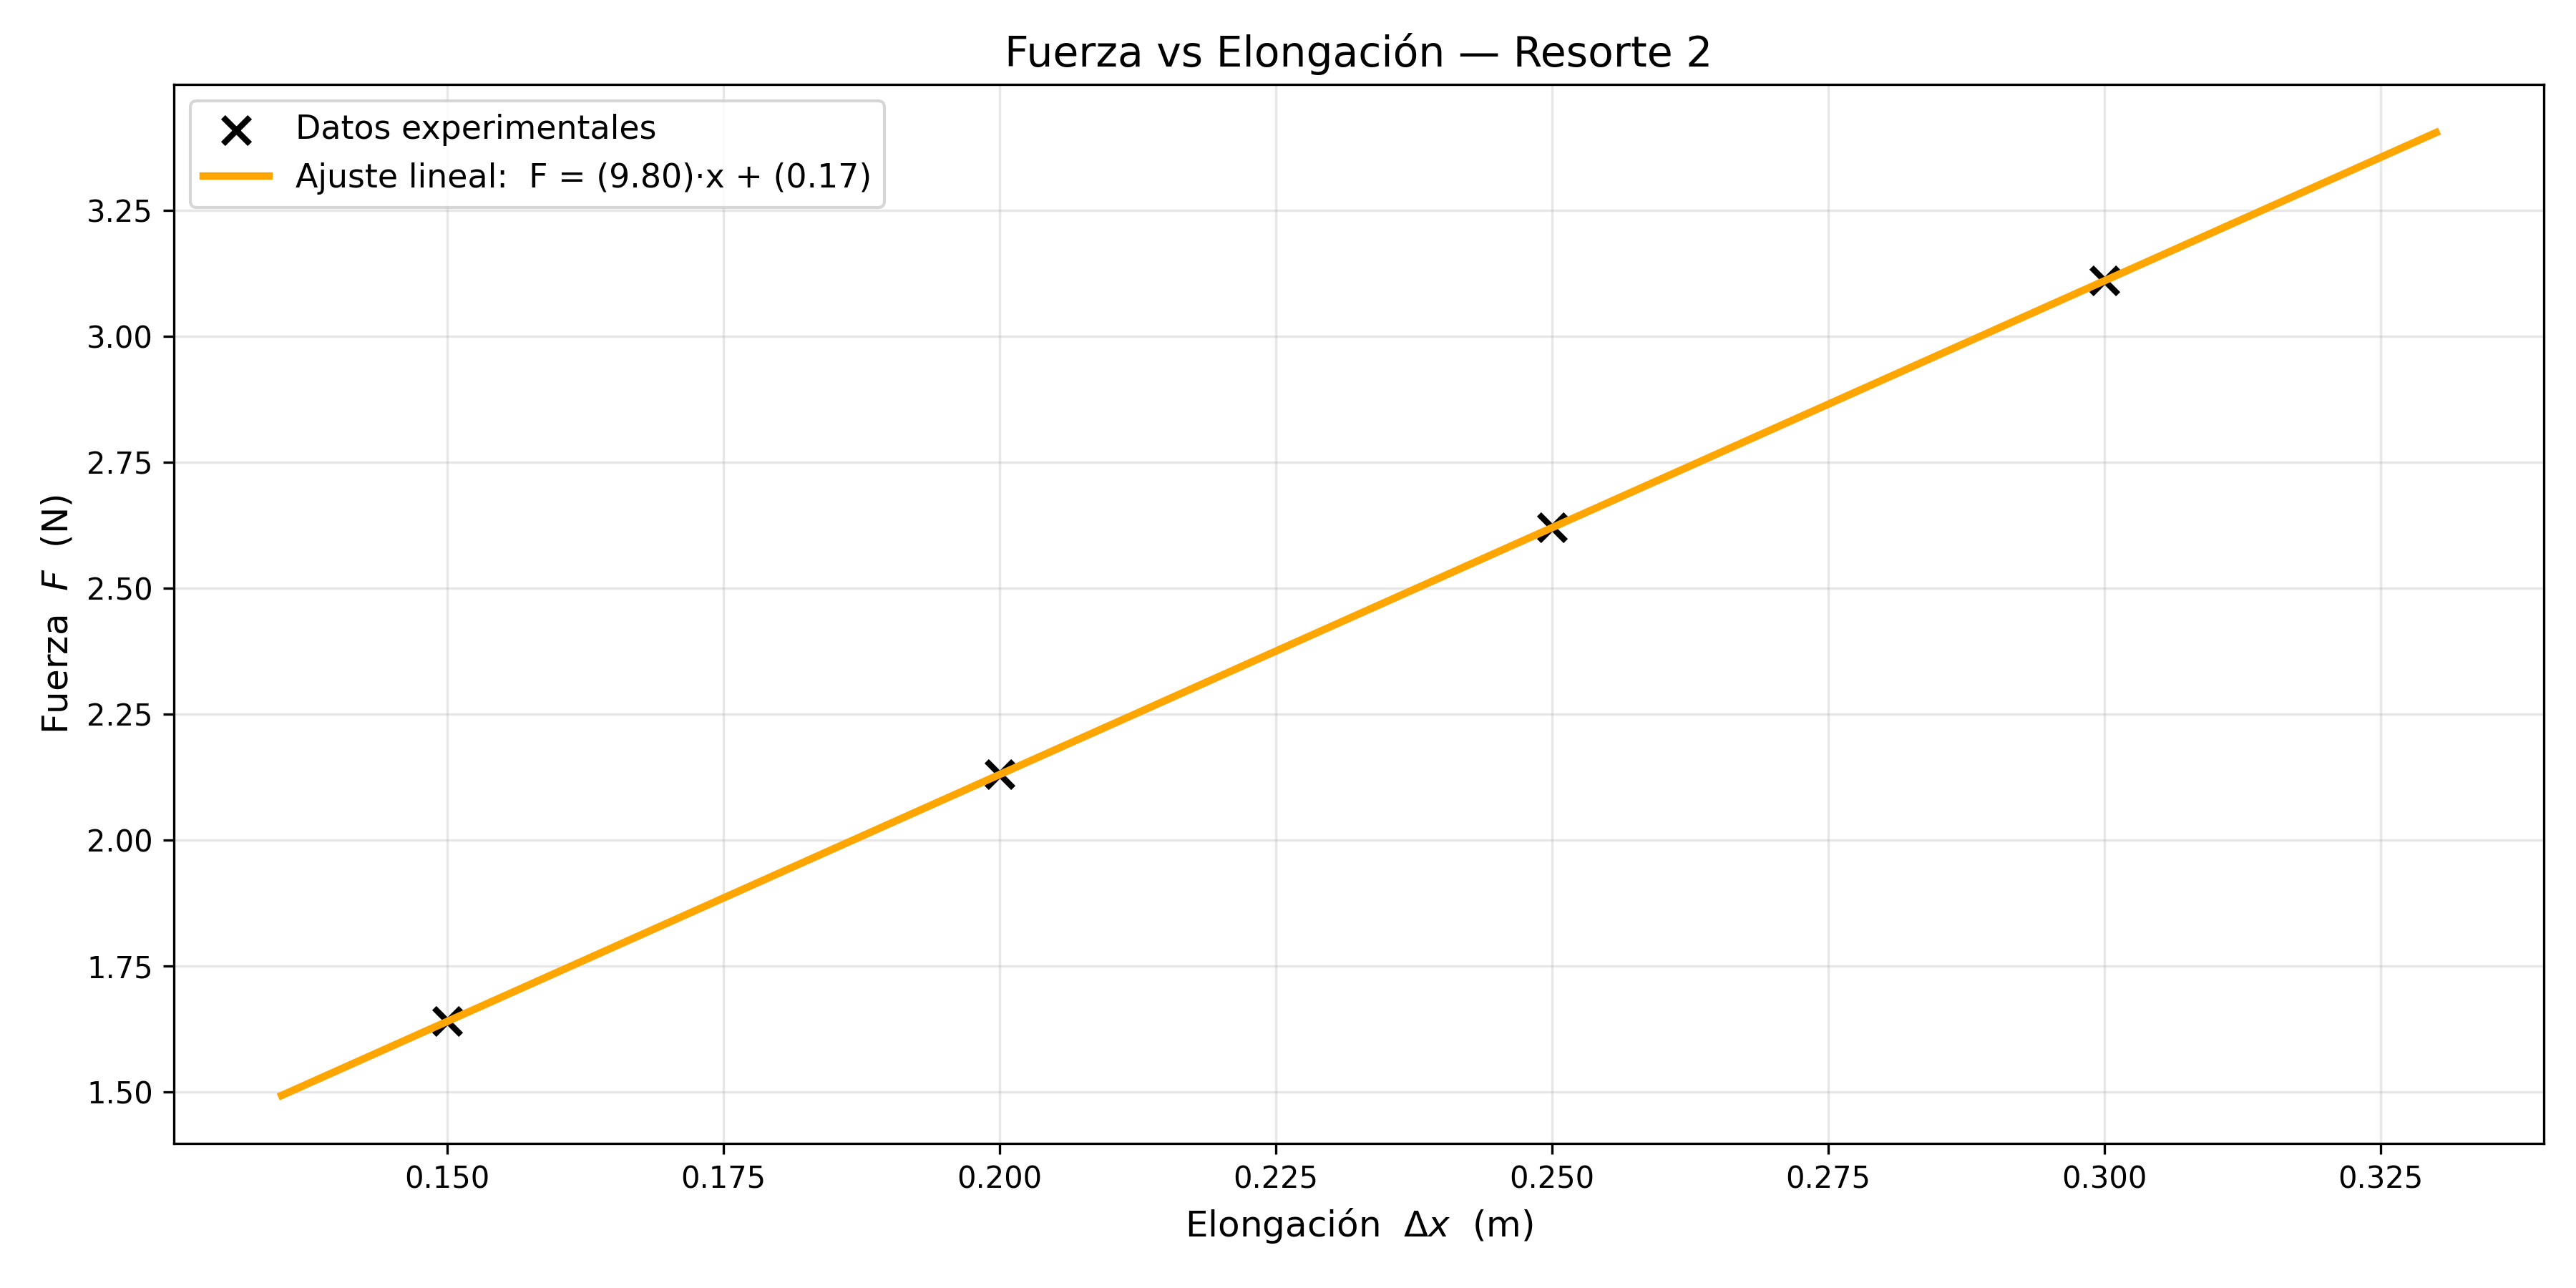
\includegraphics[width=\linewidth]{graphics/F_vs_DeltaX_resorte_2.png}
    \caption{Fuerza $F$ en función de la elongación $\Delta x$ para el resorte 2. 
    Ajuste lineal $F = k\,\Delta x + b$ con 
    $k=(9{,}800)\, \left[\mathrm{N/m} \right]$, $b=(+0{,}170)\,\left[\mathrm{N}\right]$ y $R^2=1{,}0000$.}
    \label{fig:F_vs_dx_resorte2}
\end{figure}

\subsection{¿Es la fuerza proporcional a la elongación? ¿En qué rango es válida?}

Los ajustes lineales de las Figuras~\ref{fig:F_vs_dx_resorte1} y \ref{fig:F_vs_dx_resorte2} avalan la proporcionalidad $F \propto \Delta x$ dentro de la resolución experimental para ambos resortes. En el caso del resorte 1, 
\begin{equation*}
    R^2=0.998
\end{equation*}
y la suma de los cuadrados de los residuos:
\begin{align*}
    r&=0.117
\end{align*}
esto indica que los datos se comportan casi completamente lineales, salvo una pequeña desviación en los parámetros. Esto, seguramente debido a un error en la medición. Aun así, el esquema es \emph{válido para todo el intervalo muestral}

Para el resorte 2, la linealidad se mantiene a lo largo de todo el intervalo experimental muestreado.

En ambos casos, pequeñas desviaciones a muy baja elongación son atribuibles a offset/precarga y asentamiento del sistema, sin comprometer la validez de la ley de Hooke en los rangos anteriores.

\subsection{Pendiente de la recta, dimensiones y significado físico}
Del ajuste por mínimos cuadrados:
\begin{itemize}
    \item \textbf{Para el primer resorte:}
        \begin{align*}
            k &= 29{,}953\ \left[\mathrm{\tfrac{N}{m}}\right], \\[6pt]
            b &= -0{,}339\ \left[\mathrm{N}\right],\\[6pt]
            R^2&=0.9989.
        \end{align*}
    \item \textbf{Para el segundo resorte:}
        \begin{align*}
            k &=9{,}800\ \left[\mathrm{\tfrac{N}{m}}\right], \\[6pt]
            b &= +0{,}170\ \left[\mathrm{N}\right],\\[6pt]
            R^2&=1.0000.
        \end{align*}
\end{itemize}

\begin{itemize}
\item \textbf{Dimensiones de la pendiente:} $[k] = \mathrm{N\,m^{-1}}$. 
\item \textbf{Significado físico:} $k$ es la \emph{constante elástica} del resorte (rigidez): el cociente entre la fuerza recuperadora y la elongación en el régimen lineal de la ley de Hooke.
\end{itemize}

\subsection{Ecuación de la curva obtenida del ajuste lineal}
Con los parámetros estimados para cada resorte (unidades SI), las relaciones experimentales quedan:
\begin{align*}
    F_1(\Delta x)&\approx (29.953)\,\Delta x - 0.339,\\[6pt]
    F_2(\Delta x)&\approx (9.800)\,\Delta x + 0.170,
\end{align*}
con $F$ en newtons y $\Delta x$ en metros. En un resorte ideal se esperaría $b\simeq 0$; los interceptos pequeños observados son consistentes con offset de cero, precarga o ligeros efectos de histéresis, y no alteran la estimación de la pendiente $k$.

\subsection{Fuerza elástica y constante de Hooke}
En el régimen lineal se cumple la \textbf{ley de Hooke}:
\begin{equation*}
    F = k\,\Delta x.
\end{equation*}
Experimentalmente, $k$ se identifica con la \emph{pendiente} de la recta $F$ vs.\ $\Delta x$. Para este experimento se obtiene, para cada resorte, una rigidez acorde a su comportamiento:
\begin{align*}
    k_1 &\approx 30~\mathrm{N/m}, \\[6pt]
    k_2 &\approx 9.8~\mathrm{N/m},
\end{align*}
en concordancia con los valores detallados en la subsección \emph{Pendiente de la recta, dimensiones y significado físico}. El término independiente $b$ refleja únicamente el desplazamiento de referencia y no forma parte de la ley de Hooke ideal.

% ===========================
% 7. Segunda experiencia.
% ===========================
\section{Segunda experiencia.}
\label{sec:segunda_experiencia}

En esta etapa se estudió el intercambio energético durante el movimiento oscilatorio del sistema masa–resorte. En lugar de trabajar con la elongación desde la longitud natural del resorte, se adoptó como referencia la \textbf{posición de equilibrio} $y=0$ y se registraron las \textbf{posiciones extremas} superior e inferior de la masa (véase la Figura~\ref{fig:oscilacion_resorte}). El procedimiento se realizó por separado para los \textbf{mismos dos resortes} usados en la primera experiencia (resorte 1 y resorte 2), obteniendo dos series de datos independientes.

\begin{figure}
    \centering
    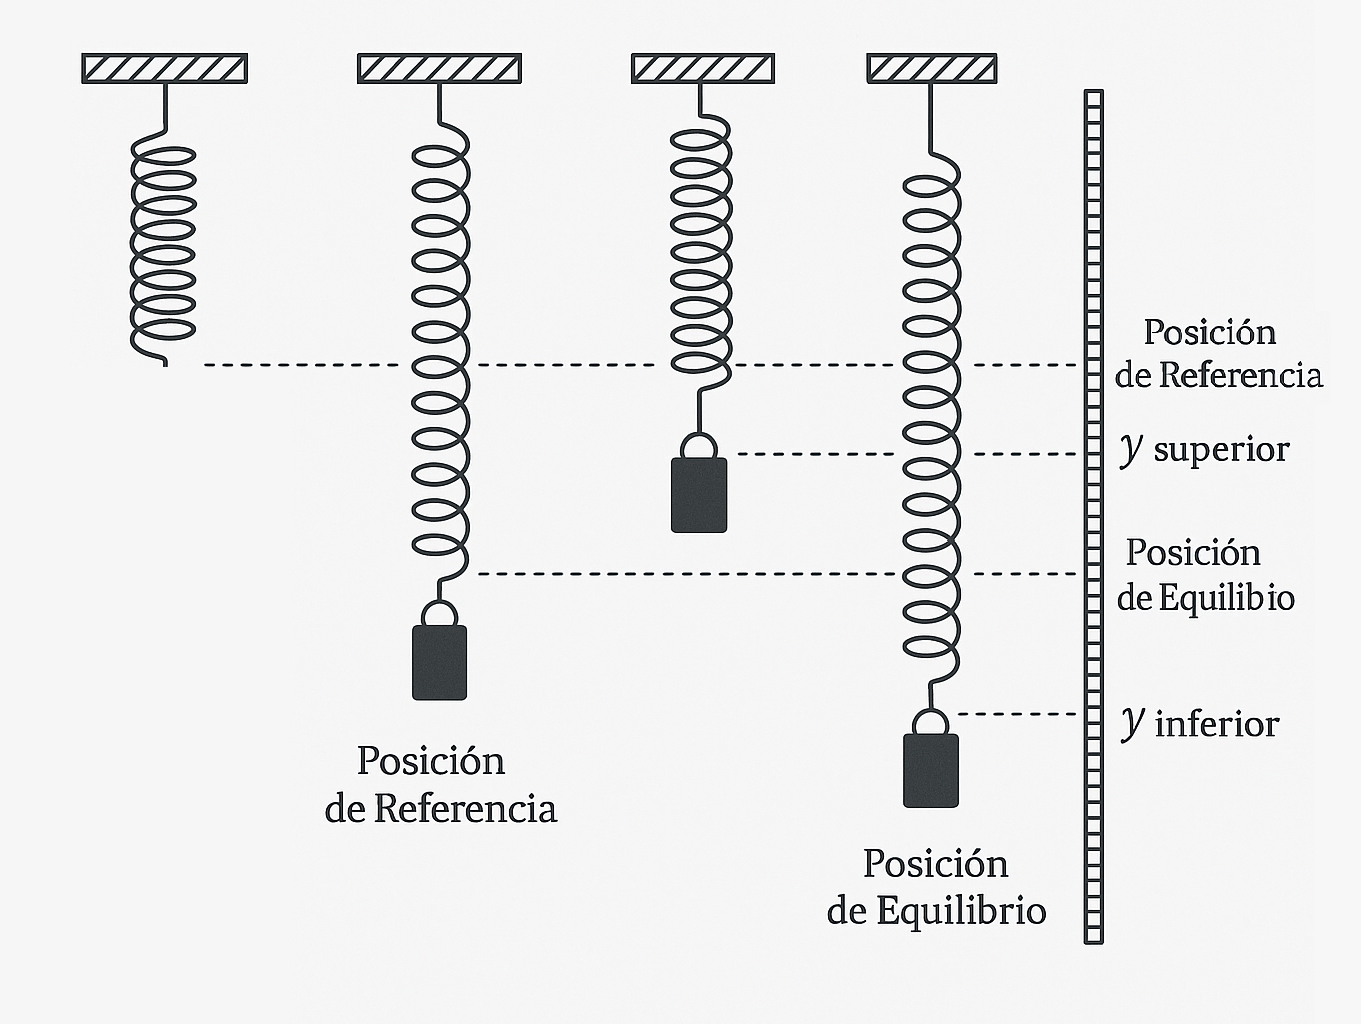
\includegraphics[width=\linewidth]{figures/figure_3.png}
    \caption{Secuencia esquemática para la toma de datos en la segunda experiencia. 
    Izquierda: \emph{posición de referencia} (resorte sin carga). Centro–izquierda: resorte con masa y \emph{posición de equilibrio} $y=0$. 
    Centro–derecha: \emph{posición extrema superior} ($y_{\text{sup}}$). Derecha: \emph{posición extrema inferior} ($y_{\text{inf}}$). 
    A la derecha se muestra la escala de lectura.}
    \label{fig:oscilacion_resorte}
\end{figure}

\subsection{Procedimiento.}
\begin{enumerate}[leftmargin=*,itemsep=2pt,topsep=2pt]
    \item Con el mismo montaje de la primera experiencia y para cada resorte por separado, se seleccionó una masa fija $m$ y se determinó cuidadosamente la posición de equilibrio del extremo libre, adoptando $y=0$ como referencia sobre la regla milimetrada (eje $y$ positivo hacia abajo, coherente con la escala).
    \item Se desplazó ligeramente la masa hacia \emph{arriba} y se liberó sin velocidad inicial apreciable. Se aguardaron 1--2 ciclos para estabilizar la amplitud. Las lecturas se realizaron a la altura de la marca para minimizar \textbf{paralaje}.
    \item Se registró la \textbf{posición extrema superior} $y_{\text{sup}}$ (por encima del equilibrio), correspondiente al máximo acercamiento del resorte a su longitud mínima.
    \item Se registró la \textbf{posición extrema inferior} $y_{\text{inf}}$ (por debajo del equilibrio), donde el resorte alcanzó su máxima extensión.
    \item Con las posiciones extremas se obtuvo la \textbf{amplitud} de oscilación:
    \begin{equation*}
        \Delta y \;=\; \frac{|y_{\text{inf}} - y_{\text{sup}}|}{2}.
    \end{equation*}
    \item Para cada corrida se evaluaron las energías, usando la \textbf{constante elástica correspondiente a cada resorte}, previamente estimada en la primera experiencia:
    \begin{align*}
        E_p^{\text{grav}} &= m g\,\Delta y,\\[4pt]
        E_p^{\text{elast}} &= \tfrac{1}{2}k_i\,(\Delta y)^2,\\[4pt]
        E_{\text{mec}} &= E_p^{\text{grav}} + E_p^{\text{elast}},
    \end{align*}
    donde $k_i$ denota $k_1$ para el \textbf{resorte 1} y $k_2$ para el \textbf{resorte 2}.
    \item Se compararon los valores de $E_{\text{mec}}$ entre corridas (para distintas amplitudes) y se discutió la \textbf{casi conservación} de la energía mecánica; discrepancias moderadas se atribuyeron a pérdidas no conservativas (rozamiento, histéresis) y a la resolución de lectura.
    \item Para cada resorte, cuando se dispuso de múltiples corridas, se promediaron las magnitudes por amplitud y se consignaron las constantes usadas ($m$, $k_i$, $g$). El cálculo numérico se documentó en el \textit{script} referido en el análisis de datos.
\end{enumerate}

\subsection{Reporte de datos.}

Las mediciones de \textbf{posiciones extremas} se realizaron conforme al procedimiento descrito: con la \textbf{posición de equilibrio} fijada como $y=0$ sobre la escala, se registraron la \emph{posición extrema superior} $y_{\text{sup}}$ y la \emph{posición extrema inferior} $y_{\text{inf}}$ en cada corrida, usando la misma regla milimetrada y una masa fija $m=\SI{0.250}{kg}$. 

Se levantaron series independientes para cada resorte bajo idénticas condiciones experimentales. Los valores recopilados se presentan por separado en los \textbf{Cuadros}~\ref{tab:oscilaciones_resorte1_parte2} (resorte 1) y~\ref{tab:oscilaciones_resorte2_parte2} (resorte 2), donde cada fila corresponde a una corrida independiente.

\begin{table}
\centering
\caption{Posiciones extremas para el \textbf{resorte 1} en oscilación libre.}
\label{tab:oscilaciones_resorte1_parte2}
\begin{tabular}{|c|c|c|}
\hline
\textbf{N$^\circ$} & $y_{\text{sup}}$ (m) & $y_{\text{inf}}$ (m) \\ \hline
1  & $0.110$ & $0.200$ \\ \hline
2  & $0.110$ & $0.203$ \\ \hline
3  & $0.110$ & $0.207$ \\ \hline
4  & $0.110$ & $0.205$ \\ \hline
5  & $0.110$ & $0.204$ \\ \hline
6  & $0.100$ & $0.210$ \\ \hline
7  & $0.100$ & $0.215$ \\ \hline
8  & $0.100$ & $0.215$ \\ \hline
9  & $0.090$ & $0.225$ \\ \hline
10 & $0.090$ & $0.223$ \\ \hline
11 & $0.090$ & $0.235$ \\ \hline
\end{tabular}
\end{table}

\begin{table}
\centering
\caption{Posiciones extremas para el \textbf{resorte 2} en oscilación libre.}
\label{tab:oscilaciones_resorte2_parte2}
\begin{tabular}{|c|c|c|}
\hline
\textbf{N$^\circ$} & $y_{\text{sup}}$ (m) & $y_{\text{inf}}$ (m) \\ \hline
1 & $0.282$ & $0.372$ \\ \hline
2 & $0.272$ & $0.386$ \\ \hline
3 & $0.262$ & $0.397$ \\ \hline
4 & $0.252$ & $0.408$ \\ \hline
5 & $0.242$ & $0.414$ \\ \hline
\end{tabular}
\end{table}


% ======================================================
% 8. Análisis de datos de la segunda experiencia.
% ======================================================

\section{Análisis de datos de la segunda experiencia.}
\label{sec:_analisis_segunda_experiencia}

\subsection{Comparación de energías potenciales}

Sea $y = 0$ la posición de equilibrio y sean $y_{\text{sup}}$ y $y_{\text{inf}}$ las posiciones extremas registradas respecto de dicha referencia (con $E_c = 0$ en ambos extremos). A partir de las mediciones directas de $y_{\text{sup}}$ y $y_{\text{inf}}$ se define la \emph{amplitud}:
\begin{equation*}
\Delta y = \frac{|y_{\text{inf}} - y_{\text{sup}}|}{2}.
\end{equation*}
Con esta $\Delta y$, las energías potenciales evaluadas en los extremos (donde $E_c=0$) se calcularon como
\begin{align*}
E_p^{\text{grav}} &= m g \,\Delta y, \\[4pt]
E_p^{\text{elast}} &= \tfrac{1}{2}k_i\,(\Delta y)^2, \\[4pt]
E_{\text{mec}} &= E_p^{\text{grav}} + E_p^{\text{elast}},
\end{align*}
donde $k_i$ denota la constante elástica del resorte correspondiente ($i=1,2$). En todos los cálculos se usaron
\begin{align*}
    m&=0.250\, [kg],\\[6pt]  
    g&=9.81\, \left[\frac{m}{s^2}\right],\\[6pt] 
    k_1&=29.953\,\left[\frac{N}{m}\right] \qquad(\text{resorte 1}),\\[6pt]
    k_2&=9.800\, \left[\frac{N}{m}\right]\qquad (\text{resorte 2}).
\end{align*}
Obsérvese que $E_p^{\text{grav}}=mg\,\Delta y$ se reporta como magnitud (siendo $\Delta y>0$), por lo que la conclusión $\Delta E_p^{\text{grav}}\simeq -\,\Delta E_p^{\text{elast}}$ es independiente de la convención de signos adoptada.

Estos resultados son magnitudes \emph{indirectas} obtenidas a partir de mediciones directas de posición y de las constantes estimadas en la primera experiencia. En un sistema ideal (sin pérdidas) se espera un intercambio complementario
\begin{equation*}
    \Delta E_p^{\text{grav}} \;\simeq\; -\,\Delta E_p^{\text{elast}},
\end{equation*}
y \emph{conservación} de la energía mecánica entre extremos de una misma corrida. Nótese que aquí se reporta, por corrida, una única $E_{\text{mec}}$ construida a partir de $\Delta y$; por ello, la igualdad 
$E_{\text{mec}}^{(\text{sup})}\simeq E_{\text{mec}}^{(\text{inf})}$ se discute de manera cualitativa (no se tabulan por separado ambas contribuciones), mientras que la consistencia del intercambio se aprecia en el orden de magnitud y el signo opuesto de $E_p^{\text{grav}}$ y $E_p^{\text{elast}}$.

Los datos procesados (SI) se presentan por separado en los 
\textbf{Cuadros~\ref{tab:energias_resorte1_parte2} y \ref{tab:energias_resorte2_parte2}} (resorte 1 y resorte 2, respectivamente). 
En ambos casos, $E_p^{\text{grav}}$ y $E_p^{\text{elast}}$ resultan de igual orden y signo opuesto, y $E_{\text{mec}}$ aumenta con la amplitud, como es esperable para oscilaciones mayores. 
Las pequeñas discrepancias se atribuyen a pérdidas no conservativas (rozamiento, histéresis) y a la resolución de lectura; el cálculo numérico utilizado se documenta en \textcolor{RoyalBlue}{\href{https://udeconce-my.sharepoint.com/:u:/g/personal/jrosas2022_udec_cl/EUfovUYl6rNPt2OGXzgADrQBErnsWO_q4iUNOX2jXK_ufg?e=lfyL2F}{este script}}.


\begin{table*}
\centering
\caption{Energías por amplitud para el \textbf{resorte 1} en la Segunda experiencia.}
\label{tab:energias_resorte1_parte2}
\begin{tabular}{|c|c|c|c|c|c|c|}
\hline
\textbf{N} & \textbf{$y_{\text{sup}}$ (m)} & \textbf{$y_{\text{inf}}$ (m)} & \textbf{$\Delta y$ (m)} & \textbf{$E_p^{\text{grav}}$ (J)} & \textbf{$E_p^{\text{elast}}$ (J)} & \textbf{$E_{\text{mec}}$ (J)} \\ \hline
1  & $0.110$ & $0.200$ & $0.045$ & $0.110$ & $0.030$ & $0.140$ \\ \hline
2  & $0.110$ & $0.203$ & $0.046$ & $0.113$ & $0.032$ & $0.145$ \\ \hline
3  & $0.110$ & $0.207$ & $0.048$ & $0.118$ & $0.035$ & $0.153$ \\ \hline
4  & $0.110$ & $0.205$ & $0.047$ & $0.116$ & $0.033$ & $0.149$ \\ \hline
5  & $0.110$ & $0.204$ & $0.047$ & $0.115$ & $0.033$ & $0.148$ \\ \hline
6  & $0.100$ & $0.210$ & $0.055$ & $0.135$ & $0.045$ & $0.180$ \\ \hline
7  & $0.100$ & $0.215$ & $0.058$ & $0.142$ & $0.050$ & $0.192$ \\ \hline
8  & $0.100$ & $0.215$ & $0.058$ & $0.142$ & $0.050$ & $0.192$ \\ \hline
9  & $0.090$ & $0.225$ & $0.067$ & $0.165$ & $0.067$ & $0.232$ \\ \hline
10 & $0.090$ & $0.223$ & $0.067$ & $0.164$ & $0.067$ & $0.231$ \\ \hline
11 & $0.090$ & $0.235$ & $0.072$ & $0.176$ & $0.078$ & $0.254$ \\ \hline
\end{tabular}
\end{table*}

\begin{table*}
\centering
\caption{Energías por amplitud para el \textbf{resorte 2} en la Segunda experiencia.}
\label{tab:energias_resorte2_parte2}
\begin{tabular}{|c|c|c|c|c|c|c|}
\hline
\textbf{N} & \textbf{$y_{\text{sup}}$ (m)} & \textbf{$y_{\text{inf}}$ (m)} & \textbf{$\Delta y$ (m)} & \textbf{$E_p^{\text{grav}}$ (J)} & \textbf{$E_p^{\text{elast}}$ (J)} & \textbf{$E_{\text{mec}}$ (J)} \\ \hline
1 & $0.282$ & $0.372$ & $0.045$ & $0.110$ & $0.010$ & $0.120$ \\ \hline
2 & $0.272$ & $0.386$ & $0.057$ & $0.139$ & $0.016$ & $0.155$ \\ \hline
3 & $0.262$ & $0.397$ & $0.067$ & $0.165$ & $0.022$ & $0.187$ \\ \hline
4 & $0.252$ & $0.408$ & $0.078$ & $0.191$ & $0.030$ & $0.221$ \\ \hline
5 & $0.242$ & $0.414$ & $0.086$ & $0.211$ & $0.036$ & $0.247$ \\ \hline
\end{tabular}
\end{table*}

\subsection{Conclusión del experimento.}

Los resultados para \textbf{ambos resortes} son \emph{consistentes con la conservación de la energía mecánica} en oscilaciones alrededor del equilibrio. Al comparar corridas con distintas amplitudes, la disminución de $E_p^{\text{grav}}$ se compensa por el aumento de $E_p^{\text{elast}}$ (y viceversa), de modo que $E_{\text{mec}}$ se mantiene aproximadamente constante dentro de la resolución experimental.

El uso de las constantes elásticas \(\,k_1\) y \(\,k_2\) \emph{propias de cada resorte}, estimadas en la primera experiencia, permite cerrar el balance energético y respalda la validez del modelo lineal de Hooke en los rangos de trabajo establecidos para cada caso. En particular, $E_{\text{mec}}$ aumenta con la amplitud de oscilación, tal como se espera para desplazamientos mayores respecto del equilibrio.

\subsection{Inferencias a partir de la conclusión.}
\begin{itemize}[leftmargin=*,itemsep=2pt,topsep=2pt]
    \item La leve no–conservatividad observada (pequeñas diferencias entre energías de corridas cercanas) indica la presencia de \textbf{disipación} por rozamiento e histéresis, además de límites de resolución en la lectura.
    \item Es imprescindible emplear la \textbf{constante elástica correspondiente a cada resorte} (\(k_1\) para el resorte 1, \(k_2\) para el resorte 2); mezclar valores de \(k\) introduce sesgos en $E_p^{\text{elast}}$ y, por ende, en $E_{\text{mec}}$.
    \item Un registro más preciso de la referencia ($y=0$) y mayor resolución en $y_{\text{sup}}$ y $y_{\text{inf}}$ reducirían el sesgo sistemático en $E_p^{\text{grav}}$ y $E_p^{\text{elast}}$; repetir lecturas por corrida y promediar mejora la estimación de \(\Delta y\).
    \item El acuerdo energético respalda el uso del \textbf{modelo lineal de Hooke} para estimar \(k_i\) y para predecir energías en \emph{pequeñas oscilaciones}. Para \textbf{amplitudes mayores}, podrían aparecer no linealidades (cambio efectivo de \(k\), histéresis más marcada), por lo que el rango utilizado resulta adecuado para el tratamiento lineal.
\end{itemize}

% ======================================================
% 9. Discusión.
% ======================================================

\section{Discusión.}

En el estudio estático (véase Sección~\ref{sec:primera_experiencia}) se verificó la relación lineal $F = k\,\Delta x + b$ para \textbf{ambos resortes}. 
Para el \textbf{resorte 1} se obtuvo $k=(29.95 \pm 0.50)\,\mathrm{N/m}$ con $R^2=0.9989$ y un pequeño $b\simeq -0.34~\mathrm{N}$, válido en el rango 
$\Delta x \in [0.18,\,0.50]~\mathrm{m}$. 
Para el \textbf{resorte 2} se obtuvo $k=(9.8 \pm 0.5)\,\mathrm{N/m}$ con $R^2\simeq 1.0000$ y $b\simeq +0.17~\mathrm{N}$, válido en 
$\Delta x \in [0.15,\,0.30]~\mathrm{m}$. 
En ambos casos, el término independiente $b$ es pequeño y compatible con un leve \emph{offset}/precarga o con la definición práctica del cero, por lo que no afecta la estimación de $k$ ni la validez de la ley de Hooke en los intervalos señalados.

En la experiencia dinámica (véase Sección~\ref{sec:segunda_experiencia}), a partir de las posiciones extremas $y_{\text{sup}}$ y $y_{\text{inf}}$ se definió 
$\Delta y=\tfrac{|y_{\text{inf}}-y_{\text{sup}}|}{2}$ y se evaluaron 
$E_p^{\text{grav}}=mg\,\Delta y$, 
$E_p^{\text{elast}}=\tfrac{1}{2}k_i(\Delta y)^2$ y 
$E_{\text{mec}}=E_p^{\text{grav}}+E_p^{\text{elast}}$, 
usando la constante elástica \emph{correspondiente a cada resorte} ($k_1$ o $k_2$). 
Se observó que $E_p^{\text{grav}}$ y $E_p^{\text{elast}}$ son de igual orden y signo opuesto en cada corrida, coherente con un \emph{intercambio complementario} y con una \emph{energía mecánica aproximadamente constante} dentro de la resolución experimental. 
Las discrepancias residuales se atribuyen a pérdidas no conservativas (rozamiento e histéresis) y a la resolución de lectura; además, $E_{\text{mec}}$ crece con la amplitud como es esperable para oscilaciones mayores alrededor del equilibrio.

Metodológicamente, la trazabilidad queda asegurada al documentar: (i) el cálculo por MCO de $k$ en la 
Sección~\ref{sec:_analisis_primera_experiencia} y (ii) el procedimiento de evaluación energética en la 
Sección~\ref{sec:_analisis_segunda_experiencia}. 
Como mejora incremental, resulta útil incluir (a) un gráfico de \emph{residuales} $F_{\text{obs}}-F_{\text{fit}}$ vs.\ $\Delta x$ para reforzar el rango lineal del ajuste estático y (b) una figura resumen con $E_p^{\text{grav}}(\Delta y)$, $E_p^{\text{elast}}(\Delta y)$ y $E_{\text{mec}}(\Delta y)$, que visualice la coherencia del balance energético para ambos resortes.

% ======================================================
% 10. Conclusiones.
% ======================================================

\section{Conclusiones.}
\begin{itemize}[leftmargin=*,itemsep=2pt,topsep=2pt]
    \item La relación estática $F=k\,\Delta x+b$ se verificó con excelente linealidad para \textbf{ambos resortes}: 
    $k_1=(29.95\pm0.50)\,\mathrm{N/m}$ en $\Delta x\in[0.18,\,0.50]~\mathrm{m}$ y 
    $k_2=(9.8\pm0.5)\,\mathrm{N/m}$ en $\Delta x\in[0.15,\,0.30]~\mathrm{m}$, con pequeños interceptos $b$ atribuibles a \emph{offset}/precarga.
    \item En el análisis dinámico, las variaciones de $E_p^{\text{grav}}$ y $E_p^{\text{elast}}$ resultaron de igual orden y signo opuesto; 
    en consecuencia, $E_{\text{mec}}$ se mantuvo aproximadamente constante entre extremos dentro de la resolución experimental, 
    evidenciando pérdidas no conservativas menores.
    \item La consistencia entre las constantes elásticas estáticas ($k_1$, $k_2$) y el balance energético dinámico respalda el \textbf{modelo lineal de Hooke} y la \textbf{conservación de la energía} para pequeñas oscilaciones alrededor del equilibrio.
    \item Para reducir discrepancias futuras se recomienda: (i) mejorar la resolución de lectura y minimizar el paralaje, 
    (ii) registrar con mayor precisión la referencia $y=0$, (iii) emplear un sensor de posición o videoanálisis para estimar $y$ con menor incertidumbre, 
    y (iv) explorar amplitudes mayores con cautela, ya que podrían emerger no linealidades (cambio efectivo de $k$ e histéresis).
\end{itemize}
\section{Apéndice: Cálculo por mínimos cuadrados}\label{sec:Apendice}

Para ajustar el modelo lineal $F(\Delta x)=k\,\Delta x + b$ a los datos $\{(\Delta x_i, F_i)\}_{i=1}^n$, se minimiza la suma de cuadrados de los residuales:
\[
\min_{k,b}\; S(k,b)\;=\;\sum_{i=1}^n \big[\,F_i - (k\,\Delta x_i + b)\,\big]^2.
\]

\paragraph{Solución cerrada.}
Definiendo las sumas con $i=1,\dots,n$, se obtiene
\begin{align*}
    k &\;=\; \frac{ n\sum \Delta x_i F_i \;-\; \left(\sum \Delta x_i\right)\!\left(\sum F_i\right) }{ n\sum \Delta x_i^2 \;-\; \left(\sum \Delta x_i\right)^2 },\\[6pt]
b &\;=\; \frac{ \sum F_i \;-\; k\sum \Delta x_i }{ n }.
\end{align*}
Con $F_i^{\text{fit}} = k\,\Delta x_i + b$, los residuales son $r_i = F_i - F_i^{\text{fit}}$.

\paragraph{Calidad del ajuste.}
El coeficiente de determinación se calcula como
\[
R^2 \;=\; 1 - \frac{\sum r_i^2}{\sum (F_i-\bar F)^2},
\qquad 
\bar F \;=\; \frac{1}{n}\sum_{i=1}^n F_i.
\]

\paragraph{Apéndice B: Implementación (script).}
El cálculo se realizó en \texttt{Python} con \texttt{NumPy}:
\begin{itemize}[leftmargin=*,itemsep=2pt,topsep=2pt]
    \item \texttt{np.polyfit(delta\_x\_m, F\_N, 1)} para estimar $k$ (pendiente) y $b$ (intercepto);
    \item \texttt{np.polyval} para evaluar $F^{\text{fit}}$;
    \item $R^2$ a partir de las sumas $\sum r_i^2$ y $\sum (F_i-\bar F)^2$.
\end{itemize}


\printbibliography

\end{document}